\chapter{Tri thức và học tăng cường}
\section{Quy trình xây dựng kho tri thức}
Kho tri thức gồm 12 ghi chú tiếng Việt biên soạn ngắn từ bảy trang chính thức NIDDK và CDC. Mỗi ghi chú lưu ID, tiêu đề, từ khóa, khái niệm, nội dung, tên nguồn, URL và ngày kiểm tra. Đây là các đoạn giải thích phục vụ học tập, không phải bản sao đầy đủ của tài liệu hướng dẫn hoặc kết quả crawl tự động toàn bộ website.

Quy trình gồm chọn chủ đề có nguồn, đọc nội dung chính thức, viết đoạn tóm lược theo phạm vi project, gán concept và liên kết nguồn, sau đó đánh giá khả năng tìm lại đoạn tương ứng. Nội dung không được thêm số liệu điều trị không xuất hiện trong nguồn. Các nguồn về xét nghiệm, HbA1c, quản lý bệnh, dinh dưỡng và vận động được liệt kê trong tài liệu tham khảo \cite{niddk_tests,niddk_a1c,niddk_manage,cdc_food,cdc_activity}.

\begin{table}[H]\centering\small
\caption{Danh mục 12 ghi chú có liên kết tới bảy trang nguồn.}
\begin{tabular}{@{}lll@{}}\toprule
ID & Chủ đề & Nguồn \\\midrule
D01 & Tiểu đường và insulin & NIDDK \\
D02 & Các loại tiểu đường & NIDDK \\
D03 & Xét nghiệm và xác nhận & NIDDK \\
D04 & Glucose lúc đói & NIDDK \\
D05 & Đường huyết thấp & CDC \\
D06 & HbA1c phản ánh thời gian dài & NIDDK \\
D07 & Giới hạn của HbA1c & NIDDK \\
D08 & Nhật ký theo dõi & NIDDK \\
D09 & Mục tiêu và thuốc & NIDDK \\
D10 & Ăn uống và khẩu phần & CDC \\
D11 & Carbohydrate & CDC \\
D12 & Vận động & CDC \\
\bottomrule\end{tabular}
\end{table}

\section{Đồ thị khái niệm local}
Đồ thị có 12 khái niệm, 8 quan hệ có hướng giữa khái niệm và 12 cạnh nối ghi chú tới khái niệm được giải thích. Ví dụ, tests nối tới fasting và a1c; a1c nối tới a1c\_limits. Cấu trúc này làm tường minh một số quan hệ giữa các phần tri thức và cung cấp một bước mở rộng khi truy xuất.

\begin{figure}[H]\centering
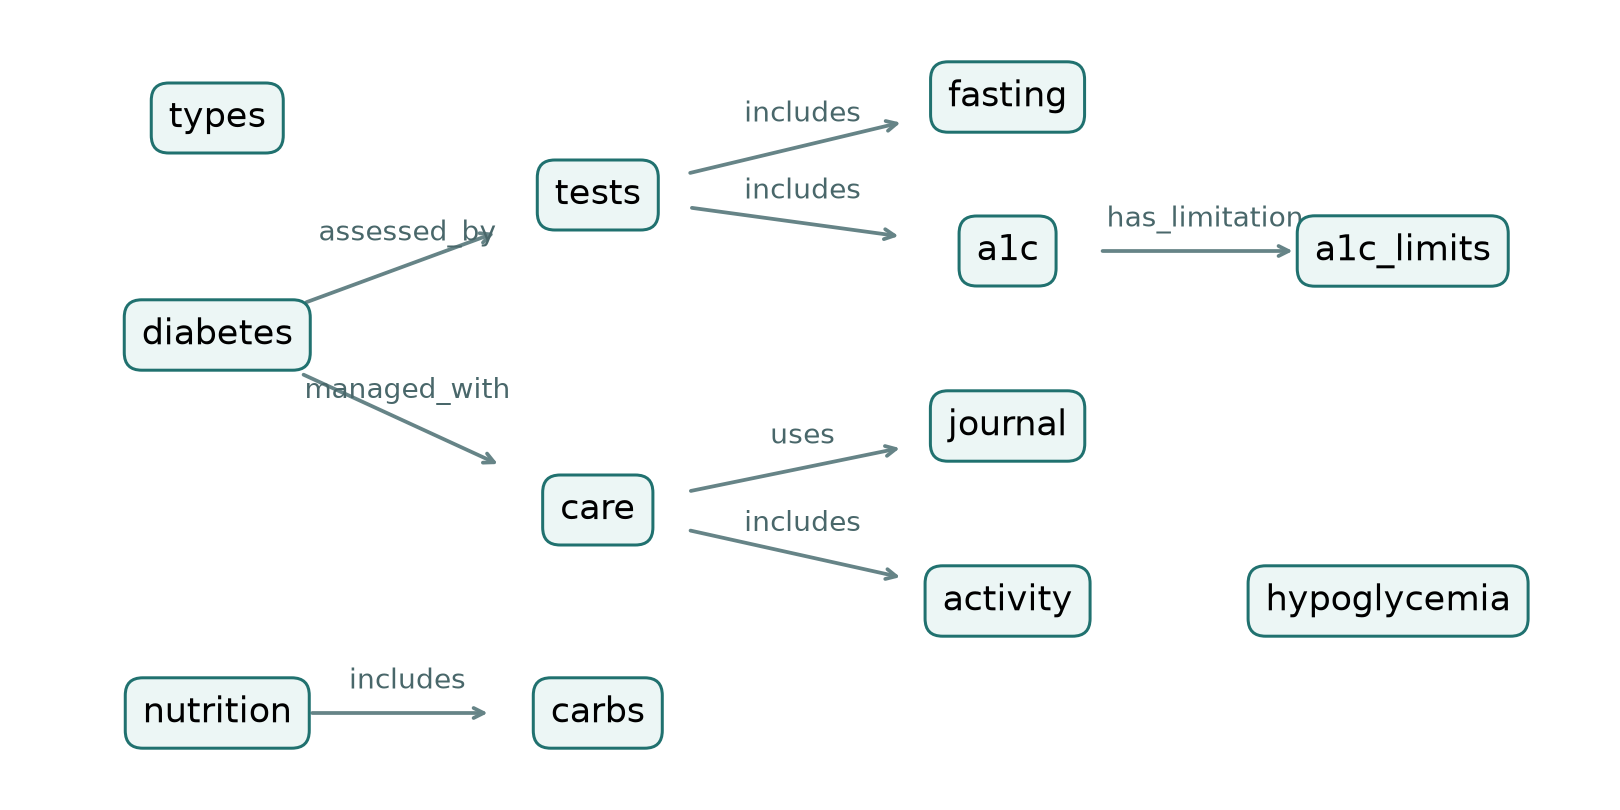
\includegraphics[width=\textwidth]{images/knowledge_graph.png}
\caption{Đồ thị 12 khái niệm và các quan hệ được biên soạn trong project. Các ghi chú D01--D12 được gắn cạnh bằng chứng trong JSON.}
\end{figure}

Graph được lưu bằng JSON và nạp trực tiếp khi ứng dụng khởi động. File \path{concept_graph.cypher} xuất nút/cạnh khái niệm để tham khảo nếu muốn tiếp tục với Neo4j; bản local không yêu cầu cài Neo4j và chưa được đánh giá trên một Neo4j server. Không gọi cách mở rộng nhỏ này là triển khai đầy đủ các phương pháp GraphRAG quy mô lớn.

\section{Truy xuất và kết xuất câu trả lời}
Văn bản được chuẩn hóa chữ thường và bỏ dấu, sau đó vector hóa TF-IDF với unigram/bigram. Corpus đầu vào cho từng ghi chú gồm tiêu đề, từ khóa và nội dung. Điểm lexical là cosine similarity giữa query và mỗi ghi chú. Alias khớp theo ranh giới từ giúp xác định các concept được nhắc trực tiếp.

Khi bật đồ thị, hệ thống mở rộng một bước theo cạnh có hướng. Ghi chú thuộc các concept trực tiếp hoặc mở rộng được cộng 0,12 vào điểm lexical. Để tránh suy ra bằng chứng chỉ vì ở gần trong graph, ứng viên phải có cosine ít nhất 0,10 nếu không khớp concept trực tiếp. Ngoài ra, ứng viên cần khớp alias hoặc có ít nhất hai token query ở tiêu đề/từ khóa sau khi bỏ một số từ chức năng.

\begin{equation}
\operatorname{score}(d,q)=\cos\bigl(v_d,v_q\bigr)+0,12\,\mathbb{1}\{C_d\cap C_q^{+}\ne\varnothing\}.
\end{equation}
Các điều kiện trên là heuristic được định nghĩa trong source; chưa có tập phát triển độc lập để chứng minh ngưỡng tối ưu. Chúng ngăn một số kết quả do trùng từ thông thường nhưng cũng có thể làm bỏ sót cách diễn đạt mới.

Tối đa ba ghi chú được trả về theo điểm, nếu bằng điểm thì theo ID. Không có ứng viên đạt thì trả insufficient\_evidence. Câu trả lời nối trực tiếp nội dung ghi chú cùng ID, còn giao diện hiển thị URL tương ứng. Đây là RAG theo kiểu truy xuất và kết xuất trích đoạn theo mẫu, không dùng LLM hoặc embedding model. Council kiểm tra tính hợp lệ của ID nhưng không chứng minh độ liên quan ngữ nghĩa của từng đoạn.

\section{Thiết kế đánh giá truy xuất}
Bộ đánh giá có 24 câu do tác giả soạn, mỗi ghi chú hai câu và một ID đích. Hit@1 kiểm tra kết quả đầu; Hit@3 kiểm tra ID xuất hiện trong ba kết quả; MRR lấy trung bình nghịch đảo thứ hạng, bằng 0 nếu không tìm thấy. Cùng bộ câu được chạy có và không có bonus đồ thị để xem đóng góp của thành phần này.

Bộ câu nhỏ và dùng từ vựng gần KB, nên không đại diện câu hỏi người bệnh ngoài thực tế. Các bài kiểm tra đã giúp phát hiện lỗi trong quá trình phát triển; vì vậy kết quả cuối là bằng chứng hồi quy và chức năng, không phải một test truy xuất độc lập chưa từng được xem. Báo cáo không dùng điểm cao để tuyên bố khả năng hiểu hội thoại y tế tổng quát.

\section{MDP nhắc ghi nhật ký}
Nhánh RL minh họa cách tác tử cải thiện chính sách qua phản hồi. Mục tiêu là cân bằng việc có bản ghi với chi phí và cảm giác mệt do thông báo. Mọi hệ số phản ứng/phần thưởng dưới đây do tác giả đặt để tạo môi trường học, không được ước lượng từ bệnh nhân hoặc thử nghiệm y khoa.

Trạng thái có dạng $s=2g+f$, trong đó $g\in\{0,1,2,3\}$ là số ngày chưa ghi, được chặn tại 3, và $f\in\{0,1\}$ là trạng thái mệt vì thông báo. Có 8 trạng thái và 3 hành động: $a=0$ không nhắc, $a=1$ nhắc ghi nhật ký, $a=2$ gửi gợi ý ghi chép ngắn. Reminder chỉ quyết định hành động trong tập này.

Xác suất ghi nhận ở bước tiếp theo được mô phỏng:
\begin{equation}
P(L=1\mid g,f,a)=\operatorname{clip}\bigl(0,40-0,07g-0,08f+b_a;\ 0,05;\ 0,95\bigr),
\end{equation}
với $b_a\in\{0;0,35;0,22\}$. Nếu có bản ghi, $g'=0$; nếu không, $g'=\min(3,g+1)$. Xác suất mệt ở ngày tiếp theo là 0,15; 0,70 hoặc 0,40 theo hành động tương ứng. Reward:
\begin{equation}
r=L-c_a-0,10g'-0,12f\mathbb{1}\{a>0\}, \qquad c_a\in\{0;0,22;0,10\}.
\end{equation}
Một policy có reward cao hơn chỉ phù hợp hơn với utility của simulator này. Reward không có đơn vị đường huyết và không đo mức cải thiện sức khỏe.

\section{Huấn luyện Q-learning}
Theo quy tắc Q-learning \cite{watkins}, tác tử cập nhật:
\begin{equation}
Q(s,a)\leftarrow Q(s,a)+\alpha\left[r+\gamma\max_{a'}Q(s',a')-Q(s,a)\right].
\end{equation}
Project dùng $\alpha=0,08$, $\gamma=0,92$, $\epsilon$-greedy với $\epsilon_e=\max(0,03;0,8\cdot0,997^e)$. Mỗi seed train có 1.800 episode, mỗi rollout 28 ngày. Đây là bài toán continuing: mốc 28 ngày chỉ là cửa sổ lấy mẫu, không phải trạng thái bệnh kết thúc, nên bước cuối vẫn bootstrap từ Q của trạng thái kế.

Năm seed train là 42--46. Mỗi policy được đánh giá greedy bằng 200 seed 10000--10199, tách khỏi seed train. Các policy đối chứng gồm không bao giờ nhắc, luôn nhắc và luật chỉ nhắc khi gap từ 2 và chưa mệt. Các lượt eval dùng cùng seed giữa policy để giảm nhiễu so sánh.

Q-table của seed 42 được dùng trong demo theo quy định trước. Project không chọn seed đạt điểm cao nhất. Độ lệch chuẩn trong bảng tổng hợp là độ biến thiên giữa năm reward trung bình của các seed train, không phải khoảng tin cậy lâm sàng.

\section{Kết hợp luật với chính sách}
Intake có thể dừng toàn bộ request trước khi Reminder được gọi. Council bác các proposal medication; action space của Reminder cũng không có hành động dùng thuốc. Khi gap/fatigue sai mã, Reminder trả needs\_input thay vì tự cắt giá trị vào miền hợp lệ. Như vậy, kết quả học được không được dùng để vượt qua giới hạn đầu vào và phạm vi hệ thống.

Project chưa học policy từ dữ liệu hành vi thật, chưa kiểm tra offline policy evaluation, chưa mô hình hóa sở thích cá nhân hoặc ràng buộc dài hạn. Việc mở rộng chỉ có ý nghĩa khi có dữ liệu và thiết kế nghiên cứu phù hợp; không suy rộng từ bảng Q nhỏ sang chính sách chăm sóc thực tế.
